\chapter{模拟退火法}

之前我们的随机算法都有一个特性,即我们清楚随机变量的分布情况,能够用AR
法等手段进行服从指定分布的抽样,从而提高随机算法的效率和精度。同时,我
们的模拟目标往往是随机变量的某个数字特征,因此可以通过大数定律逼近。这
一章我们将随机算法扩展到优化领域。同时要面对上述前提失效的问题。本章的
内容基于参考书\cite{Kanglishan1994}。

\section{组合优化问题}
我们知道有很多离散优化问题,是
属于NP(Non-deterministic Polynomial )的,其中最著名的一个可能就是
TSP(Traveling Salesman Problem)问题,它的一种描述如下:给定$n$个城市
和每两个城市间的距离(无向完全图,有权边),选择一条线路,使得每个城市
只经过一次且仅有一次,并最终回到起点。求能完成这个遍历的总路径长度最短。
对于完全图,我们用邻借矩阵(adjacency matrix)$D = [d_{ij}]$来表示全部
城市,其中$d_{ij}$表示城市$i$和$j$之间的距离。显然,$d_{ij}$满足:
\begin{enumerate}
\item $d_{ij} \geq 0, 1 \leq i, j \leq n$;
\item $d_{ii} = 0, 1 \leq i \leq n$;
\item $d_{ij} = d_{ji}, 1 \leq i, j \leq n$;
\item $d_{ij} + d_{jk} \geq d_{ik}, 1 \leq i, j, k \leq n$.
\end{enumerate}
一个解可以表达为一个循环排列
$$
\pi = (\pi_1, \pi_2, \cdots, \pi_n),
$$
表示路径
$$
\pi_1 \to \pi_2 \to \cdots \to \pi_n,
$$
其中$\pi_i \in \{1, 2, \cdots, n\}, i = 1, 2, \cdots, n$表示各个城市
的编号,显然对可行解,有$i \neq j$,有$\pi_i \neq \pi_j$。若记$S$为全体
可行解,则易知
\begin{equation}
  |S| = \frac{(n - 1)!}{2},
\end{equation}
这是一个随$n$增加指数增长的数值,因此对于较大的$n$不太可能用遍历穷举的
方式来寻找最优解。这里目标函数可以表示为
\begin{equation}
  f(\pi) = \sum_{i = 1}^n d_{\pi_i, \pi_{i + 1}},
\end{equation}
这里约定$\pi_{n + 1} = \pi_1$。整个优化问题按组合优化的约定,可以表达为
\begin{equation}
  \min f(\pi_i), \pi_i \in S.
\label{eq::TSP_opt}
\end{equation}
而优化问题(\ref{eq::TSP_opt})的解则定义为:

\begin{definition}{\hei 全局最优解} 称$\pi^* \in S$为问题(\ref{eq::TSP_opt})
  的全局最优解,或简称最优解,若$\forall \pi_i \in S$,有
  $$
   f(\pi^*) \leq f(\pi_i).
  $$
\end{definition}

作为一个典型的NP问题,对每一个可行解(存在的路径),我们都可以迅速得到
总路径长度(多项式时间)。然而,求最短路径本身却至今没有什么太好的确定
性算法。在这种情况下,随机搜索算法又一次被提到桌面上讨论。然而现在出现
新的困难,和积分问题不同,最优解是一个非常孤立的偶然事件,同时分布上也
没有明显的规律(或者我们无法先验地获知它的分布情况),如果完全在$S$全
空间随机投点,去碰一个偶然事件,那么收敛速度甚至收敛性本身都很有问题。
针对这种未知分布的情况,我们得改变我们的抽样技巧。但首先,我们先观察一
下$S$的结构(总是要尽可能获取背景信息)。

\begin{definition}{\hei $2$-变换邻域}
对于$S$中的一个解
$$
\pi = \{\pi_1, \pi_2, \cdots, \pi_{p - 1}, \pi_p, \pi_{p + 1},
\cdots, \pi_{q - 1}, \pi_q, \pi_{q + 1}, \cdots, \pi_n\},
$$
称
$$
N_2(p, q): \pi \to \pi', p < q
$$
为$2$-变换,如果
$$
\pi'= \{\pi_1, \pi_2, \cdots, \pi_{p - 1}, \pi_q, \pi_{q - 1},
\cdots, \pi_{p - 1}, \pi_p, \pi_{q + 1}, \cdots, \pi_n\}.
$$
对$\forall \pi_i \in S$,称$S_i$为$\pi_i$的$2$-变换邻域,若$S_i \subseteq S$,
且$\forall \pi_j \in S_i$,$\pi_j$可由$\pi_i$经一次$2$-变换得到。
\end{definition}

类似的,我们还可以定义$k$-变换,以及$k$-变换邻域。但注意到$\forall i,
j \in S$,我们都可以用至多$n - 2$次$2$-变换将二者互换。所以从考虑可行
解之间关系角度,$2$-变换在很多场合也够用了。有了邻域,我们可以进一步提出:

\begin{definition}{\hei 局部最优解}
  记$\pi^* \in S$的邻域为$S^*$,若$\forall \pi_i \in S^*$,有
  $$
  f(\pi_i) \geq f(\pi^*), 
  $$
  则称$\pi^*$为优化问题(\ref{eq::TSP_opt})的局部最优解。
\end{definition}

现在我们给出一个用于求解一般组合优化问题的伪代码:

\begin{minipage}[!ht]{0.8\textwidth}
\vspace{3ex}
\refstepcounter{alg}
\label{alg::LSA}
\begin{center}
 算法 \arabic{chapter}.\arabic{alg} {\hei 组合优化问题的局部搜索算法} 
\end{center}
\small
\begin{tabular}{lll}
  \hei 输入&i0&初值\\
  \hei 输出&&局部最优解
\end{tabular}
\begin{lstlisting}[style = python]
def local_search(i0):
    i = i0
    while (i不是局部最优解):
        从i的邻域Si中选取一个可行解j
        if f(j) < f(i):
            i = j
    return i
\end{lstlisting}
\end{minipage}

这个算法很通用,但也很没用。它只能提供局部最优解,对于TSP这样显然要求
全局最优的问题,它显得很无力。(TSP算法有实用的离散算法,详见谈之奕主
  讲课程《组合优化》。)我们这里考虑能否使用随机搜索的手段,使这个算法
摆脱局部最优解的困扰,但同时我们又要利用局部最优性。因为在没有其他任何
信息的时候,局部最优性显然提供了一个邻域内的有效索方向。这里可以考虑的
几个关键点是:
\begin{enumerate}
  \item 我们在邻域内每次都做一个随机选取,即总是从$S_i$中随机抽取一个
    $j$,作为下一步尝试的可行解。比如具体在TPS问题中,可以通过随机抽取
    $p$和$q$来进行$2-$变换邻域内的随机抽取;
  \item 当存在邻域内的可行解$j$满足$f(j) > f(i)$时,也应该有一定概率用
    $j$去代替$i$,也就是说应该保留一定概率让解往非局部最优的方向行走,
    这样才能留下脱离局部最优解的可能性。具体这个概率应该服从什么分布?
    这个是我们接下去要讨论的问题;
  \item 再引入了上述随机搜索之后,算法\ref{alg::LSA}的终止判定不再适用,
    应该相应修改为若当前解$i$在一个指定的步数$N$($N >> 1$)都不再变化
    时,算法终止。
\end{enumerate}

由于缺乏关键过程2,我们现在还无法写出这个算法,但大致思想框架已经形成。

\section{Metropolis准则}

Metropolis是一个人名,他是一个物理学家。由于工作的缘故,他是首批接触到
计算机的人之一,因此也为计算机模拟计算的早期研究作出了杰出贡献。当时的
计算机还非常低效,不太可能进行高维大范围的随机抽样。而Metropolis在求解
一组原子结构的最低能量状态时,提出了后来被称为Metropolis准则的模拟方法。

\begin{figure}[!ht]
\centering
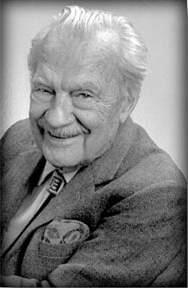
\includegraphics[width=0.3\textwidth]{images/Nicholas.PNG}
\caption{Nicholas Metropolis,1915 - 1999,希腊裔美国物理学家,曼哈顿
  计划的参与者}
\label{fig::game}
\end{figure}

物质在从液态变成固态时,系统的能量是整体降低的。粒子(我们这里不区分原
  子、分子)从能流动到被固定在一个有限范围振动,物质的结构性加强,
能量降低,熵减少。这里温度是刻画粒子状态的一个统计量。在宏观意义上,它
和粒子系统的能量是正相关的。同时在宏观上,我们可以通过控制外界温度,来
影响系统的温度,进而影响系统状态。比如对于液体,我们降低温度,它会凝固
成固体。这一过程称为退火。实践和理论研究都指出,温度降低的过程对最终形
成的固体的性态是有影响的。如果温度急剧下降,那么粒子系统来不及和周围环
境进行充分的能量交换,从而导致粒子尚未进入到能量最低态就进入固体状态,
因此形成的固体物质结构较为脆弱。而如果能控制温度缓慢下降,使粒子系统整
体能量和外界交换均匀充分,那么粒子系统能量降低到一个最低值时,趋于稳定,
此时形成的固体,结构更加坚固。物理学家通过理论分析和实验,得到一系列关
于物质能量和熵条件的结果,我们这里不再详述,有兴趣同学自行阅读参考书。
而1953年Metropolis在前人工作的基础上,提出了一种用于模拟系统能量最低态的
随机采样准则:若系统在状态$i$时的能量为$E_i$,在$i$的邻域内随机选取
$j\neq i$,且状态$j$的能量为$E_j$。若$E_j < E_i$,则称状态$j$为“重要
状态”,否则,若$E_j > E_i$,则以
\begin{equation}
  r = e^{\frac{E_i - E_j}{kT}}
  \label{eq::Metropolis}
\end{equation}
的概率决定$j$是否为重要状态。也就是说,产生一个服从$U(0, 1)$的随机数
$\xi$,若$\xi < r$,则接受$j$为重要状态,否则舍弃。在一次随机尝试中,
如果$j$是重要状态,则用$j$代替$i$成为当前状态。公式
(\ref{eq::Metropolis})来源于统计物理学中的Gibbs分布,而$k$是
Boltzmann常数,而$T$是温度。受到启发,Kirkpatrick在1983年
\cite{KirkpatrickGelattVecchi83}将这种基于物质退火过程模拟的思
想引入了组合优化领域,提出了模拟退火算法(Simulated
  Annealing Algorithm)。回顾我们之前考虑局部随机搜索算法时尚未解决的
第2步,即解$i$应该以怎样的概率转移到解$j$?根据模拟退火法,这个转移概
率可以写作:
\begin{equation}
  P_t\{i \to j\} = \left\{
  \begin{array}{ll}
    1, & f(j) \leq f(i)\\
    e^{\frac{f(i) - f(j)}{t}}, &\mbox{其它}.
  \end{array}
  \right.
  \label{eq::SAA_metro}
\end{equation}
这里将所有参数吸收为一个$t > 0$,显然$t$越大,则转移概率越高;而$t$越
小,转移概率越低。这与物质退火的直观一致。我们在执行算法时,可以在初期
将$t$设的较大,然后慢慢降低$t$,最终使状态最终在一个能量低点稳定。

现在我们可以给出基于Metropolis准则的随机局部搜索算法,也即模拟退火算法
的伪代码。

\begin{minipage}[!ht]{0.8\textwidth}
\vspace{3ex}
\refstepcounter{alg}
\label{alg::SA}
\begin{center}
 算法 \arabic{chapter}.\arabic{alg} {\hei 模拟退火算法} 
\end{center}
\small
\begin{tabular}{lll}
  \hei 输入&i0&初值\\
  &t0&初始温度\\
  &L0&初始随机搜索步长,即在初始温度下的随机搜索次数。\\
  \hei 输出&&数值最优解
\end{tabular}
\begin{lstlisting}[style = python]
def simulated_annealing(i0, t0, L0):
    k = 0
    i = i0
    while (1):
        for l = 1 to Lk:
            从i的邻域Si中选取一个可行解j
            if f(j) < f(i):
                i = j
            else:
                xi = random(0, 1)
                if xi < exp((f(i) - f(j))/tk):
                    i = j
        k = k + 1
        调整Lk
        调整tk
        若满足终止条件,跳出循环
    return i
\end{lstlisting}
\end{minipage}

这仍然只是一个框架式算法思路。如何调整Lk,tk,以及如何制定终止条件,既
有理论上的讨论,也要根据实际问题具体分析。但我们这里先给出一个关于模拟
退火法的收敛性的统计学特性。

\begin{definition}{\hei 平稳分布}
  给定组合优化问题$(S, f)$,和一个相关的邻域结构。对固定的$t$值做足够
  多的基于Metropolis准则(\ref{eq::SAA_metro})变换之后,全体可行解的
  分布服从
  \begin{equation}
    P\{X = i\} := q_i(t) = \frac{e^{-\frac{f(i)}{t}}}{N_0}
    \label{eq::Metro_Gibbs_dis}
  \end{equation}
  其中$X$是表示当前解的随机变量,而
  \begin{equation}
    N_0(t) = \sum_{i \in S} e^{-\frac{f(j)}{t}}
    \label{eq::Metro_Gibbs_dis_regular}
  \end{equation}
  是归一化因子。式(\ref{eq::Metro_Gibbs_dis})称为平稳分布。
\end{definition}
模拟退火法的当前解服从平稳分布是一个假设。在这个假设下,我们有

\begin{theorem}{}
  若组合优化问题$(S, f)$的当前解服从平稳分布,则
  \begin{equation}
    \lim_{t \to 0}q_i(t) := q_i^* = \frac{1}{|S_{\mathrm{opt}}|}\chi_{\mathrm{opt}}.
  \end{equation}
  其中$S_{\mathrm{opt}}$表示最优解集合(不唯一),而$\chi_{\mathrm{opt}}$
  则表示可行解$i$是最优解的特征函数:
  \begin{equation}
    S \to \{0, 1\}, \chi_{\mathrm{opt}}(i) = \left\{\begin{array}{ll}
    1, & i \in S_{\mathrm{opt}},\\
    0, &\mbox{其它}.
    \end{array}\right.
  \end{equation}
\end{theorem}

这个定理表明,如果每个$t$至都能达到平稳分布,那么算法能收敛到全局最优解。先看证明。

\begin{proof}
  对$\forall a \geq 0$,有
  \begin{equation}
    \lim_{x \to 0} e^{\frac{a}{x}} = \left\{
    \begin{array}{ll}
      1, & a = 0,\\
      0, & a < 0.
    \end{array}
    \right.
  \end{equation}
  所以
  \begin{eqnarray*}
    \lim_{t \to 0}q_i(t) & = & \lim_{t \to 0}  \frac{e^{-\frac{f(i)}{t}}}
        {\sum_{j \in S} e^{-\frac{f(j)}{t}}} \\
        & = & \lim_{t \to 0} \frac{\frac{e^{f_{\mathrm{opt}} - f(i)}}{t}}
        {\sum_{j \in S} e^{\frac{f_{\mathrm{opt}} - f(j)}{t}}} \\
        & = & \lim_{t \to 0}\frac{1}{\sum_{j \in S} e^{\frac{f_{\mathrm{opt}} - f(j)}{t}}}
        \chi_{\mathrm{opt}}(i)
        + \lim_{t \to 0} \frac{e^{\frac{f_{\mathrm{opt}} - f(i)}{t}}}
        {\sum_{j \in S}e^{\frac{f_{\mathrm{opt}} - f(j)}{t}}}\chi_{\mathrm{opt}}(i)\\
        & = & \frac{1}{|S_{\mathrm{opt}}|} \chi_{\mathrm{opt}}(i) + 0. 
  \end{eqnarray*}
\end{proof}

下面列出一些关于模拟退火法的重要统计学特征,具体的证明参见文献\cite{Aarts1989Simulated}。

\begin{definition}{\hei 平衡时的期望目标函数}
  \begin{equation}
    E_t(f) := \langle f \rangle_t = \sum_{i \in S}f(i)q_i(t).
    \label{eq::Metro_esp_t_f}
  \end{equation}
\end{definition}

\begin{definition}{\hei 平衡时的期望平方目标函数}
  \begin{equation}
    E_t(f^2) := \langle f^2\rangle_t = \sum_{i \in S}f^2(i)q_i(t).
    \label{eq::Metro_esp_t_f2}
  \end{equation}
\end{definition}

\begin{definition}{\hei 平衡时的目标函数方差}
  \begin{equation}
    Var_t(f) := \sigma_t^2 = \sum_{i \in S}(f(i) - \langle f\rangle_t)^2q_i(t)
    = \langle f^2\rangle_t - \langle f\rangle_t^2.
    \label{eq::Metro_t_variation}
  \end{equation}
\end{definition}

\begin{definition}{\hei 平衡时的熵}
  \begin{equation}
    S_t(f) := \sum_{i \in S} q_i(t) \log q_i(t).
    \label{eq::Metro_t_entropy}
  \end{equation}
\end{definition}

\begin{theorem}{}
  \begin{equation}
    \frac{\partial}{\partial t}\langle f\rangle_t = \frac{\sigma_t^2}{t^2},
  \end{equation}
  \begin{equation}
    \frac{\partial}{\partial t}S_t = \frac{\sigma_t^2}{t^3},
  \end{equation}
\end{theorem}

\begin{theorem}{}
  \begin{equation}
    \lim_{t \to \infty} \langle f\rangle_t := \langle f\rangle_\infty
    = \frac{1}{|S|}\sum_{i \in S} f(i).
  \end{equation}
  \begin{equation}
    \lim_{t \to 0} \langle f\rangle_t := f_{\mathrm{opt}}.
  \end{equation}
  \begin{equation}
    \lim_{t \to \infty} \sigma_t^2 := \sigma_\infty^2 = \frac{1}{|S|}
    \sum_{i \in S}(f(i) - \langle f\rangle_\infty)^2.
  \end{equation}
  \begin{equation}
    \lim_{t \to 0} \sigma_t^2 = 0.
  \end{equation}
  \begin{equation}
    \lim_{t \to \infty} S_t := S_\infty = \log |S|.
  \end{equation}
  \begin{equation}
    \lim_{t \to 0} S_t := S_0 = \log |S_{\mathrm{opt}}|.
  \end{equation}
\end{theorem}

有上述定理可知,若在每个$t$时刻都能满足平稳分布,则模拟退火法的期望目
标函数和熵分别单调减少至$f_{\mathrm{opt}}$和$\log |S_{\mathrm{opt}}|$.

\begin{theorem}{} 设$(S, f)$表示某个组合优化问题,
  且$S_{\mathrm{opt}} \neq S$(非平凡). 并设$q_i(t)$为相关$t$时刻平稳分布,则
  \begin{enumerate}
  \item $\forall i \in S_{\mathrm{opt}}$,有
    \begin{equation}
      \frac{\partial}{\partial t}q_i(t) < 0;
    \end{equation}
  \item $\forall i \notin S_{\mathrm{opt}}$, $f(i) \geq \langle f\rangle_\infty$,有
    \begin{equation}
      \frac{\partial}{\partial t} q_t(i) > 0;
    \end{equation}
  \item $\forall i \notin S_{\mathrm{opt}}$, $f(i) < \langle f\rangle_\infty$,则
    $\exists \tilde{t}_t > 0$, 使
    \begin{equation}
      \frac{\partial}{\partial t} q_i(t) \left\{
      \begin{array}{ll}
        > 0, & t < \tilde{t}_i, \\
        = 0, & t = \tilde{t}_i, \\
        < 0, & t > \tilde{t}_i.
      \end{array}
      \right.
    \end{equation}
  \end{enumerate}
  \label{thm::Metro_q_t}
\end{theorem}

由定理\ref{thm::Metro_q_t}知,模拟退火法找到一个整体最优解的概率随$t$
的减少而单调增大;且对每个非整体最优解,都存在$\tilde{t}_i$,使得当$t
< \tilde{t}_i$时,当前解为该解的概率随$t$的减少而单调减少。


